\chapter{质点运动学}

\section*{A 组}
\vspace{0.3cm}
\textbf{1-1} 精密测定重力加速度 $g$ 的一种方法是在真空容器中竖直向上抛出一个小球，测出小球抛出后两次经过某竖直位置 $A$ 的时间间隔 $T_{A}$ 和两次经过另一竖直位置 $B$ 的时间间隔 $T_{B}$ . 若已知 $B$ 在 $A$ 的上方 $h$ 处，试求重力加速度 $g$.

\vfill

\textbf{1-2} 在地面上方同一位置分别以 $v_{1}, v_{2}$ 为初速度，先后向上抛出两个小球，第2个小球抛出后经过 $\tau$ 时间与第1个小球相遇。改变两球抛出的时间间隔，便可改变 $\tau$ 值。设 $v_{A}, v_{B}$ 已选定，且 $v_{1} < v_{2}$ ，试求 $\tau$ 的最大值。


\vfill

\newpage

\textbf{1-3} 图 1-2 所示一系列光滑斜面的顶端与底端间的水平距离同为 $l$，倾角 $\phi$ 在 $0 \sim 90^{\circ}$ 间连续取值，让小球从斜面顶端自静止下滑到底端，所经时间记为 $T(\phi)$ .

(1) 试求 $T(\phi)$ 的最小值 $T_{\min}$ .


(2) 取 $\phi=30^{\circ},45^{\circ},60^{\circ}$ ，分别画出小球沿斜面运动速度 $v$ 随时间 $t$ 的变化曲线，并计算各自平均值 $\bar{v}$ .


\begin{center}
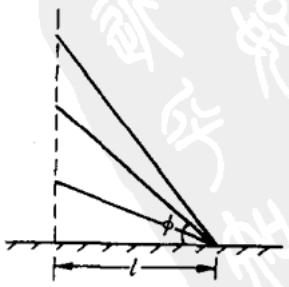
\includegraphics[width=0.2\textwidth]{figures/图1_2.jpg}
\end{center}

\vfill

\textbf{1-4} 飞机着陆后为尽快停下,采用尾部“降落伞”制动. t=0 刚着陆时的速度大小记为 $v_{0}$ , 坐标取成 $x = 0$ . 假设滑行过程中加速度为 $a_{x} = -\beta v_{x}^{2}$ , 其中 $\beta$ 是正的常量, 试求速度 $v_{x}$ 随位置 $x$ 的变化关系.

1-5 在 $x$ 轴上运动的某质点，加速度与位置的关系为 $a_x = -\omega^2 x$ ，其中 $\omega$ 是正的常量. 已知 $t = 0$ 时，质点位于 $x_0 > 0$ 处，速度 $v_0 \neq 0$ ，试求质点位置 $x$ 随时间 $t$ 的变化关系.

\vfill

\newpage

\textbf{1-6} 小球从同一位置以相同的初速率 $v_{0}$ ，在同一竖直平面上朝着不同方向斜抛出去，如果抛射角 $\theta$ 可在 $0 \sim \pi$ 范围内连续变化，试问各轨道最高点连成的曲线是什么类型曲线？


\vfill

\textbf{1-7} 一位足球运动员踢出的球具有初速率 25 m/s, 今在球门正前方 50 $m$ 处欲将球踢进球门. 为防止守门员将球挡住, 他选择进球位置在正前方球门水平横梁下方 50 cm 之内区域. 已知横梁高为 2.44 $m$, 试问他应在什么倾角范围将球踢出?


\vfill

\newpage

\textbf{1-8} 一地面雷达观察者正从屏幕上监视由远处投来的一抛射体. 某时刻, 他得到的信息显示: 抛射体达到了最高点且具有水平速度 $v; v$ 的方向线与观察者、抛射体位于同一竖直平面; 抛射体与观察者之间的距离为 $l$ ; 观察者到抛射体连线与水平面的夹角为 $\theta$ .


(1) 预测抛射体落地点与观察者间的水平距离 $d$;


(2) 预测抛射体能否越过观察者的头顶?


\vfill

\textbf{1-9} 离地高 $h$ 的大厅吊灯爆炸成碎片，朝各个方向射出，初速度同为 $v_{0}$ . 设吊灯离屋顶和墙较远，碎片不会与之相撞；再设地面铺有毛毯，碎片落地后不会反弹. 试将每一碎片运动斜交地分解成沿其初速 $v_{0}$ 方向的匀速直线运动和静止开始的竖直向下自由落体运动，以此求解地面上碎片分布区域的半径 $R$.

\vfill

\newpage

\textbf{1-10} 质点在 $xy$ 平面上运动, $t = 0$ 时刻, 位于 $x_0 = A, y_0 = 0$ , 速度的两个分量各是 $v_{x0} = 0, v_{y0} = B\omega$ , 任意 $t$ 时刻加速度的两个分量各是 $a_x = -A\omega^2 \cos \omega t, a_y = -B\omega^2 \sin \omega t$ , 其中 $A, B, \omega$ 都是常量, 试求质点运动轨道.


\vfill

\textbf{1-11} 查找有关数据,估算下述各量的大小:


(1) 氢原子中电子绕核圆运动的加速度值(绝对值);


(2) 学生匀速骑自行车直线行进时, 车轮边缘点的加速度值;


(3) 以太阳为参考物, 地面上的实验室因地球自转和公转而具有的最大可能的加速度值.


\vfill

\newpage

\textbf{1-12} 半径同为 $R$ 的两个几何球面开始时互相重合, 今使其中一个球面固定, 另一个球面从 t=0 开始匀速平动, 速度大小为 $v_{0}$ .

(1) 试求两球面刚好完全分离的时刻 $t_{e}$ ;

(2) 试求 $0 < t < t_{e}$ 时刻, 两球面交线长度收缩率(单位时间内长度缩短量) $\gamma$ ;

(3) 试求 $0 < t < t_{e}$ 时刻, 两球面交点在第一球面大圆上作圆运动的向心加速度 $a_{心}$ 和切向加速度 $a_{切}$ .


\vfill

\textbf{1-13} 四质点 $A, B, C, D$ 在同一平面上运动。每一时刻， $A$ 速度总对准 $B$ ，速度大小为常量 $u; B$ 速度总对准 $C$ ，速度大小同为 $u; C$ 速度总对准 $D$ ，速度大小同为 $u; D$ 速度总对准 $A$ ，速度大小同为 $u$ 。某时刻， $A, B, C, D$ 恰好逆时针方向按序位于各边长为 $l$ 的正方形四个顶点上，试求此时 $A$ 的加速度 $a$ 和 $A$ 的运动轨道在此位置的曲率半径 $\rho$ .


\vfill

\newpage

\textbf{1-14} 采用运动学方法, 求解曲线 $y = \mathrm{e}^x$ 的曲率半径随 $x$ 的分布 $\rho(x)$ .

\vfill

\textbf{1-15} 在极坐标系中,质点沿着图 1-8 所示的直线以恒定的速度 $v_{0}$ 运动.


(1) 结合图中给出的参量, 写出直线轨道方程 $r-\theta$ ;

(2) 写出质点速度分量 $v_{r}, v_{\theta}$ 与质点角位置 $\theta$ 的关系，再依据加速度分量计算公式，验证 $a_{r}=0, a_{\theta}=0$ .


\begin{center}
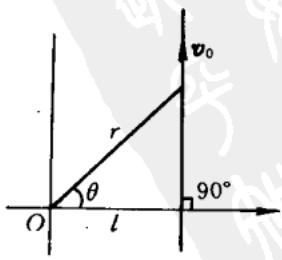
\includegraphics[width=0.2\textwidth]{figures/图1_8.jpg}
\end{center}

\vfill

\newpage

\textbf{1-16} 以椭圆一个焦点 $F$ 为原点，沿半长轴方向设置极轴，椭圆的极坐标方程是 $r = r_0 / (1 + e\cos \theta)$ . 设所给椭圆的半长轴为 $A$ ，半短轴为 $B$ ，且 $F$ 如图所示，位于椭圆中心 $O$ 的右侧.

(1) 确定参量 $r_{0}, e$ 与 $A$, $B$ 的关系；


(2) 若质点以 $\theta=\omega t$ 方式沿椭圆运动，试导出 $v_{\theta}, a_{\theta}$ 与质点角位置 $\theta$ 的关系.

\begin{center}
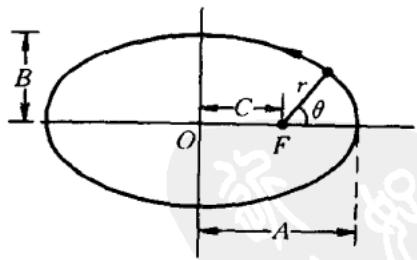
\includegraphics[width=0.2\textwidth]{figures/图_1_9.jpg}
\end{center}

\vfill

\textbf{1-17} 平面上有三个动点 $A, B, C, t = 0$ 时刻三者连线构成边长为 $l$ 的等边三角形. 取三角形中心 $O$ 为极坐标系原点, 取 $t = 0$ 时刻 $O$ 到 $A$ 的连线为极轴, 如图所示. 若 $A, B, C$ 均在此平面内作匀速率运动, 速率同为 $u$ , 过程中 $A$ 始终朝着 $B$ 运动, $B$ 始终朝着 $C$ 运动, $C$ 始终朝着 $A$ 运动, 试求 $A$ 点运动轨道.


\begin{center}
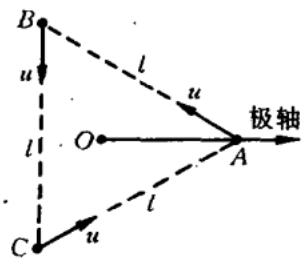
\includegraphics[width=0.2\textwidth]{figures/图1_10.jpg}
\end{center}


\vfill

\newpage

\textbf{1-18} 极坐标系中方程$r = A (1 - \cos \theta)$,对应一条心脏线,如图所示,试求心底 $P$ 处曲率半径 $\rho$ .


\begin{center}
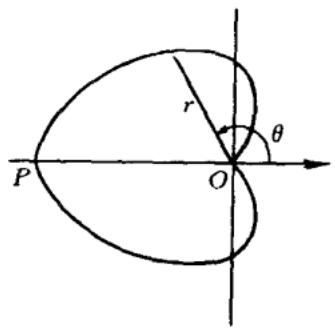
\includegraphics[width=0.2\textwidth]{figures/图1_12.jpg}
\end{center}

\vfill

\textbf{1-19} 半径 $R$ 的细圆环在半径几乎同为 $R$ 的固定光滑圆柱面外侧面上随意运动, 试求环的自由度.


\vfill

\newpage

\textbf{1-20} 在 $Oxy$ 坐标平面上有一个正三角形和一个正方形, 正三角形和正方形的每条边长相同, 它们的方位如图所示. 现在建立一个活动的 $O'x'y'$ 坐标平面, 它的坐标原点开始时位于正三角形的上顶点, 而后 $Q'$ 点沿着正三角形的三条边绕行一周. 绕行时, $x'$ 轴始终与 $x$ 轴平行, $y'$ 轴始终与 $y$ 轴平行. 试在图中清楚、准确地画出正四边形相对 $O'x'y'$ 坐标平面运动而形成的区域的边界线.

\begin{center}
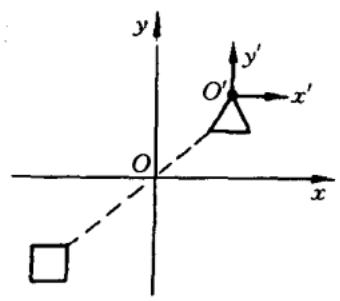
\includegraphics[width=0.2\textwidth]{figures/图1_13.jpg}
\end{center}


\vfill

\textbf{1-21} 树上一个苹果离地面高 2.5 $m$, 小孩在距树 1.5 $m$ 处, 从 1.5 $m$ 高度对准苹果抛出一颗小石子的同时, 苹果自由落下. 不计空气阻碍作用, 试问小石子抛出的速度 $v$ 为何值时能击中苹果?


\vfill

\newpage

\textbf{1-22} 风自西向东吹, 风速 $u$ 不变, 一架军用飞机相对于静止大气的飞行速率为恒定的 $v_{0}$ . 设飞机在城市上空沿水平圆轨道巡航飞行, 建立自西向东的 $x$ 轴, 将飞机相对于圆心的径矢与 $x$ 轴夹角记为 $\phi$ , 试求连续的圆轨道飞行条件及轨道速率 $v$ 与方位角 $\phi$ 的关系.


\vfill

\textbf{1-23} 刚性的圆环静止在地面上, t=0 时刻开始以恒定的角加速度 $\beta$ 沿直线作纯滚动. 试求任意 t>0 时刻, 环上最高点的加速度大小 $a_{上}$ 与最低点的加速度大小 $a_{下}$ 之比值.


\vfill

\newpage

\textbf{1-24} 细杆 $ABC$ 在一竖直平面上靠着一个台阶放着, $A$ 端可沿着水平地面朝台阶运动, 细杆不离开台阶边沿. 当 $ABC$ 杆与水平地面夹角为图 1-16 所示的 $\phi$ 时, 杆的 $B$ 点恰好位于台阶边沿上, 而且 $C$ 端运动速度值恰为 $A$ 端运动速度值的 2 倍, 试求 $BC$ 长与 $AB$ 长的比值 $\alpha$ .


\begin{center}
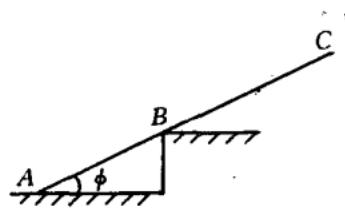
\includegraphics[width=0.2\textwidth]{figures/图1_16.jpg}
\end{center}



\vfill

\textbf{1-25} 4 根长度同为 $l$ 的细杆, 用铰链首尾相接, 组成一个菱形 $ABCD$ , 放在某水平面上, 如图所示. 设 $A$ 端固定, $C$ 端沿着 $A$ , $C$ 连线方向运动, 当 $\angle A$ 恰为 $90^{\circ}$ 时, $C$ 端速度为 $v$ , 加速度为 $a$ , 试求此时 $B$ 端的加速度大小 $a_{B}$ .

\begin{center}
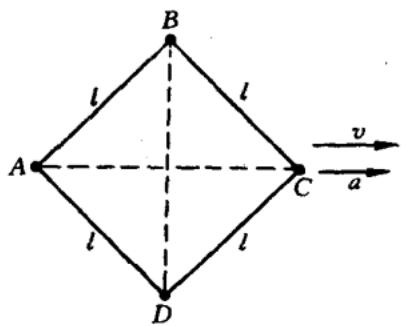
\includegraphics[width=0.2\textwidth]{figures/图1_18.jpg}
\end{center}

\vfill

\newpage

\section*{B 组}
\vspace{0.3cm}
\textbf{1-26} 在某竖直平面上有一固定的光滑直角三角形细管道 $ABC$ ，小球从顶点 $A$ 沿斜边轨道静止出发自由滑到端点 $C$ 所需时间，恰好等于小球从 $A$ 静止出发自由地经两条直角边轨道滑到 $C$ 所需时间。此处假设竖直轨道 $AB$ 与水平轨道 $BC$ 的交接处为极小的圆弧，可确保小球无碰撞地拐弯，且拐弯时间可略。将 $AB, BC, AC$ 的长分别记作 $L_1, L_2, L_3$ ，试求三者比例关系。

在此直角三角形范围内可构建一系列如图所示的光滑折线轨道，每一轨道由若干竖直与水平部分交接而成，交接处有极小圆弧（作用同前），轨道均从 $A$ 到 $C$ ，且不越出该直角三角形边界，试求小球在各条轨道中，自静止出发从 $A$ 滑行到 $C$ 所经时间的上限 $T_{\mathrm{max}}$ 与下限 $T_{\mathrm{min}}$ 之比.


\begin{center}
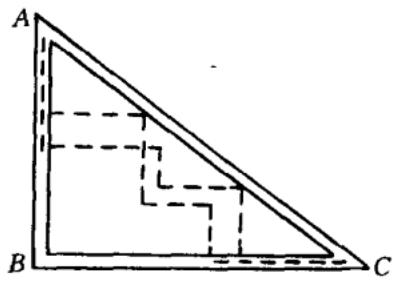
\includegraphics[width=0.2\textwidth]{figures/图1_20.jpg}
\end{center}


\vfill

\textbf{1-27} 如图所示, $A$ 和 $B$ 是两个相同的刚性小球, 开始时 $A$ 和 $B$ 在同一竖直线上, 各自距水平地面的高度分别是 $h_{A}$ 和 $h_{B}$ , 且 $h_{A} > h_{B}$ . 令两球同时从静止自由落下, 而后若两球相碰则彼此交换速度, 若其中一球与地面相碰, 则以原速率反向弹回. 要求 $A$, $B$ 不会与地面一起发生三体碰撞, 试讨论系统形成周期运动的条件.

\begin{center}
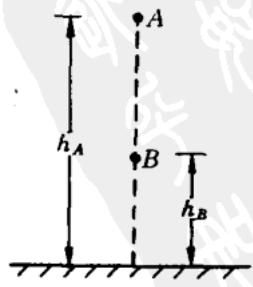
\includegraphics[width=0.2\textwidth]{figures/图_1_22.jpg}
\end{center}

\vfill

\newpage

\textbf{1-28} 长 $L$ 的均匀弹性绳 $AB$ 自由伸直地放在光滑水平桌面上, 绳的 $A$ 端固定. $t = 0$ 时, 一小虫开始从 $A$ 端出发以相对绳的匀速度 $u$ 在绳上朝 $B$ 端爬去, 同时绳的 $B$ 端以匀速度 $v$ 沿绳伸长方向运动, 试求小虫爬到 $B$ 端的时间 $T$ .


\vfill

\textbf{1-29} 某人用两手做3个球的抛球、接球、传球游戏. 过程中左手接住空中落下的一个球, 再传递给右手; 右手接过小球, 并将小球斜向上抛出. 假设每只手中至多只留有一个小球, 左手接球点高度与右手抛球点高度相同, 每个小球离开右手后的升高量均达 $H$ , 小球互相不碰撞, 试求系统运动周期 $T$ .


\vfill

\newpage

\textbf{1-30} （1）加速度恒定的运动称为匀加速运动，试证质点的匀加速运动必定是直线运动或者是平面曲线运动,后一种称为匀加速平面曲线运动,简称匀加速曲线运动.


（2）作匀加速曲线运动的质点，在时间 $t_1 = 1\mathrm{s}, t_2 = 2\mathrm{s}, t_3 = 3\mathrm{s}$ 时刻，分别位于空间 $A, B, C$ 点。已知 $\overline{AB} = 8\mathrm{m}, \overline{BC} = 6\mathrm{m}$ ，且 $AB \perp BC$ ，试求质点运动加速度 $\pmb{a}$ 。

\vfill

\textbf{1-31} 小物体以初速 $v_{0}$ 、倾角 $\theta$ 斜抛出去，在空气中运动因受阻力而获得与速度 $v$ 反向的附加加速度 $-\gamma v$ ，其中 $\gamma$ 是一个正的常量，试解析给出小物体的运动轨道曲线.


\vfill

\newpage

\textbf{1-32} 设由 $y=y(x)$ 表述的平面曲线，在讨论区域内处处连续，而且 $y' = dy/dx, y'' = d^{2}y/dx^{2}$ 也处处存在并连续，试用运动学方法求解曲率半径分布 $\rho(x)$ .

\vfill

\textbf{1-33} 如图所示, 岸高 $h$, 人用绳经滑轮拉船靠岸. 若绳与水面夹角为 $\theta$ 时, 人左行速度为 $v_{0}$ , 加速度为 $a_{0}$ (均未必是常量), 试求此时船的左行速度 $v$ 和加速度 $a$.
\begin{center}
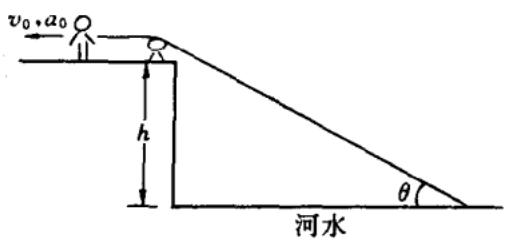
\includegraphics[width=0.2\textwidth]{figures/图1_25.jpg}
\end{center}


\vfill

\newpage

\textbf{1-34} 极坐标系中的对数螺线可表述为 $r=r_{0}e^{\alpha\theta}$ ，试用运动学方法导出曲率半径分布 $\rho(r)$ .

\vfill

\textbf{1-35} 空间光滑连续曲线上取三个点, 可确定一个平面, 这三个点无限靠近时确定的极限平面记为 $\sigma$ , 曲线上由这三个点的两个端位点界定的无穷小曲线段必定都在 $\sigma$ 平面内, 并可逼近处理成无穷小圆弧段, 圆半径便是这一空间曲线在此位置处的曲率半径.


等距螺旋线的曲率半径必定处处相同,试用运动学方法,求解旋转圆半径和螺距分别为 $R$ 和 $H$ 的等距螺旋线的曲率半径 $\rho$ .


\vfill

\newpage

\textbf{1-36} 如图所示, 轰炸机 $A$ 以速度 $v_{1}$ 作水平匀速飞行, 飞行高度为 $H$.


(1) 为使自由释放的炸弹击中地面目标 $B$，应在距 $B$ 多远的水平距离 $L$ 处投弹？（2）在地面上与 $B$ 相距 $D$ 处有一高射炮 $C$，在 $A$ 释放炸弹同时发射炮弹，为使炮弹能击中飞行中的炸弹，试问炮弹初速 $v_{2}$ 至少为多大？若 $v_{2}$ 取最小值，炮弹发射角 $\gamma$ 为多大？
\begin{center}
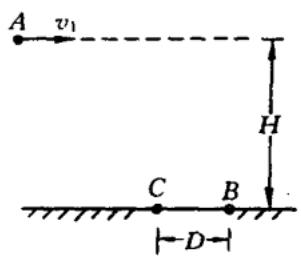
\includegraphics[width=0.2\textwidth]{figures/图1_30.jpg}
\end{center}

\newpage


\textbf{1-37} 惠更斯等时摆.

半径 $R$ 的轮子在水平直线 MN 上方纯滚动, 轮子边缘上任意点 $P$ 的运动轨迹不妨称为上滚轮线. 如图所示, 将上滚轮线绕 MN 向下翻转 $180^{\circ}$ , 成为下滚轮线. 下滚轮线也可看成 $R$ 轮子在下方沿直线 MN 纯滚动时轮子边缘点 $P$ 的运动轨迹.

沿下滚轮线设置光滑轨道, 小球在轨道内侧除最低点外任意一处从静止自由滑下, 可形成周期性的往返运动(摆动), 惠更斯已证得摆动周期 $T$ 与小球初始位置无关, 后人将此种摆称为惠更斯等时摆. 试在认知等时性前提下, 求出以 $R$ 为参量的 $T$ 算式.

\begin{center}
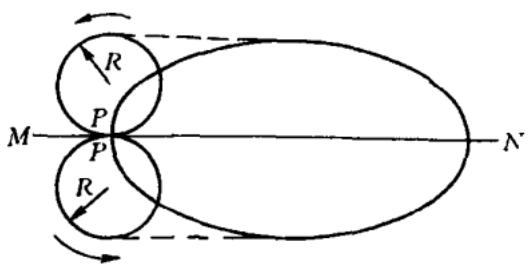
\includegraphics[width=0.2\textwidth]{figures/图1_32.jpg}
\end{center}


